\documentclass[american, titlepage, oneside]{ntnuthesis}

% Front page
\title{Identification of Multiple Simultaneous Pipeline Leaks Using Inlet-Outlet Steady-State Measurements}
\shorttitle{Multi Leak Identification}
\author{Anders Mørk}
\shortauthor{A. Mørk}
\date{\today}

\addbibresource{thesis.bib}

\newglossaryentry{ell}{
    name={$\ell$},
    description={length of pipe}
}

\newglossaryentry{z}{
    name={$z$},
    description={spatial coordinate along the pipe, $0 \leq z \leq \ell$}
}

\newglossaryentry{qz}{
    name={$q(z)$},
    description={volumetric discharge/flow at position $z$}
}

\newglossaryentry{hz}{
    name={$h(z)$},
    description={piezometric head at position $z$}
}

\newglossaryentry{n}{
    name={$n$},
    description={number of leaks in the pipe}
}

\newglossaryentry{zi}{
    name={$z_i$},
    description={location of the $i$-th leak, for notation purposes $z_0=0$ and $z_{n+1}=\ell$}
}

\newglossaryentry{tildeqi}{
    name={$\tilde q_i$},
    description={discharge/flow through the $i$-th leak}
}

\newglossaryentry{ci}{
    name={$c_i$},
    description={discharge coefficient of the $i$-th leak}
}

\newglossaryentry{U}{
    name={$U$},
    description={head loss function}
}

\newglossaryentry{q0}{
    name={$q_0$},
    description={flow at the pipe inlet}
}

\newglossaryentry{ql}{
    name={$q_\ell$},
    description={flow at the pipe outlet}
}

\newglossaryentry{h0}{
    name={$h_0$},
    description={head at the pipe inlet}
}

\newglossaryentry{hl}{
    name={$h_\ell$},
    description={head at the pipe outlet}
}

\newglossaryentry{qi}{
    name={$q_i$},
    description={constant steady-state flow in pipe segment $[z_i,z_{i+1})$}
}

\newglossaryentry{Li}{
    name={$L_i$},
    description={length of the $i$-th pipe segment}
}

\newglossaryentry{hi}{
    name={$h_i$},
    description={head at the $i$-th leak location, for notation purposes $h_{n+1}=h_\ell$}
}

% delete??
\newglossaryentry{y}{
    name={$y^{(j)}$},
    description={measurement set containing $\{h_0^{(j)},h_{\ell}^{(j)},q_0^{(j)},q_{\ell}^{(j)}\}$ and corresponding to the $j$-th operating point}
}

\newglossaryentry{y0}{
    name={$y_0^{(j)}$},
    description={Inlet measurements of flow and head for the $j$-th operating point}
}

\newglossaryentry{yl}{
    name={$y_{\ell}^{(j)}$},
    description={Outlet measurements of flow and head for the $j$-th operating point}
}

\newglossaryentry{m}{
    name={$m$},
    description={number of steady-state operating point measurements}
}

\newglossaryentry{M}{
    name={$\mathcal M$},
    description={complete collection of measurements}
}

\newglossaryentry{M0}{
    name={$\mathcal M_0$},
    description={set of inlet measurements}
}

\newglossaryentry{Ml}{
    name={$\mathcal M_\ell$},
    description={set of outlet measurements}
}

\newglossaryentry{theta}{
    name={$\theta$},
    description={hydraulic resistance coefficient for a pipe}
}

\newglossaryentry{dwfric}{
    name={$f$},
    description={Darcy--Weisbach friction factor}
}

\newglossaryentry{x}{
    name={$\mathbf{x}$},
    description={vector containing leak parameters}
}

\newglossaryentry{phi}{
    name={$\phi^{(j)}$},
    description={collection of state variables corresponding to the $j$-th operating point}
}

\makeatletter
\renewenvironment{theglossary}
  {\begin{longtable}{@{}p{0.12\linewidth}p{0.82\linewidth}@{}}}
  {\end{longtable}}
\makeatother

\begin{document}

%\includepdf[pages=-]{master_agreement.pdf}
%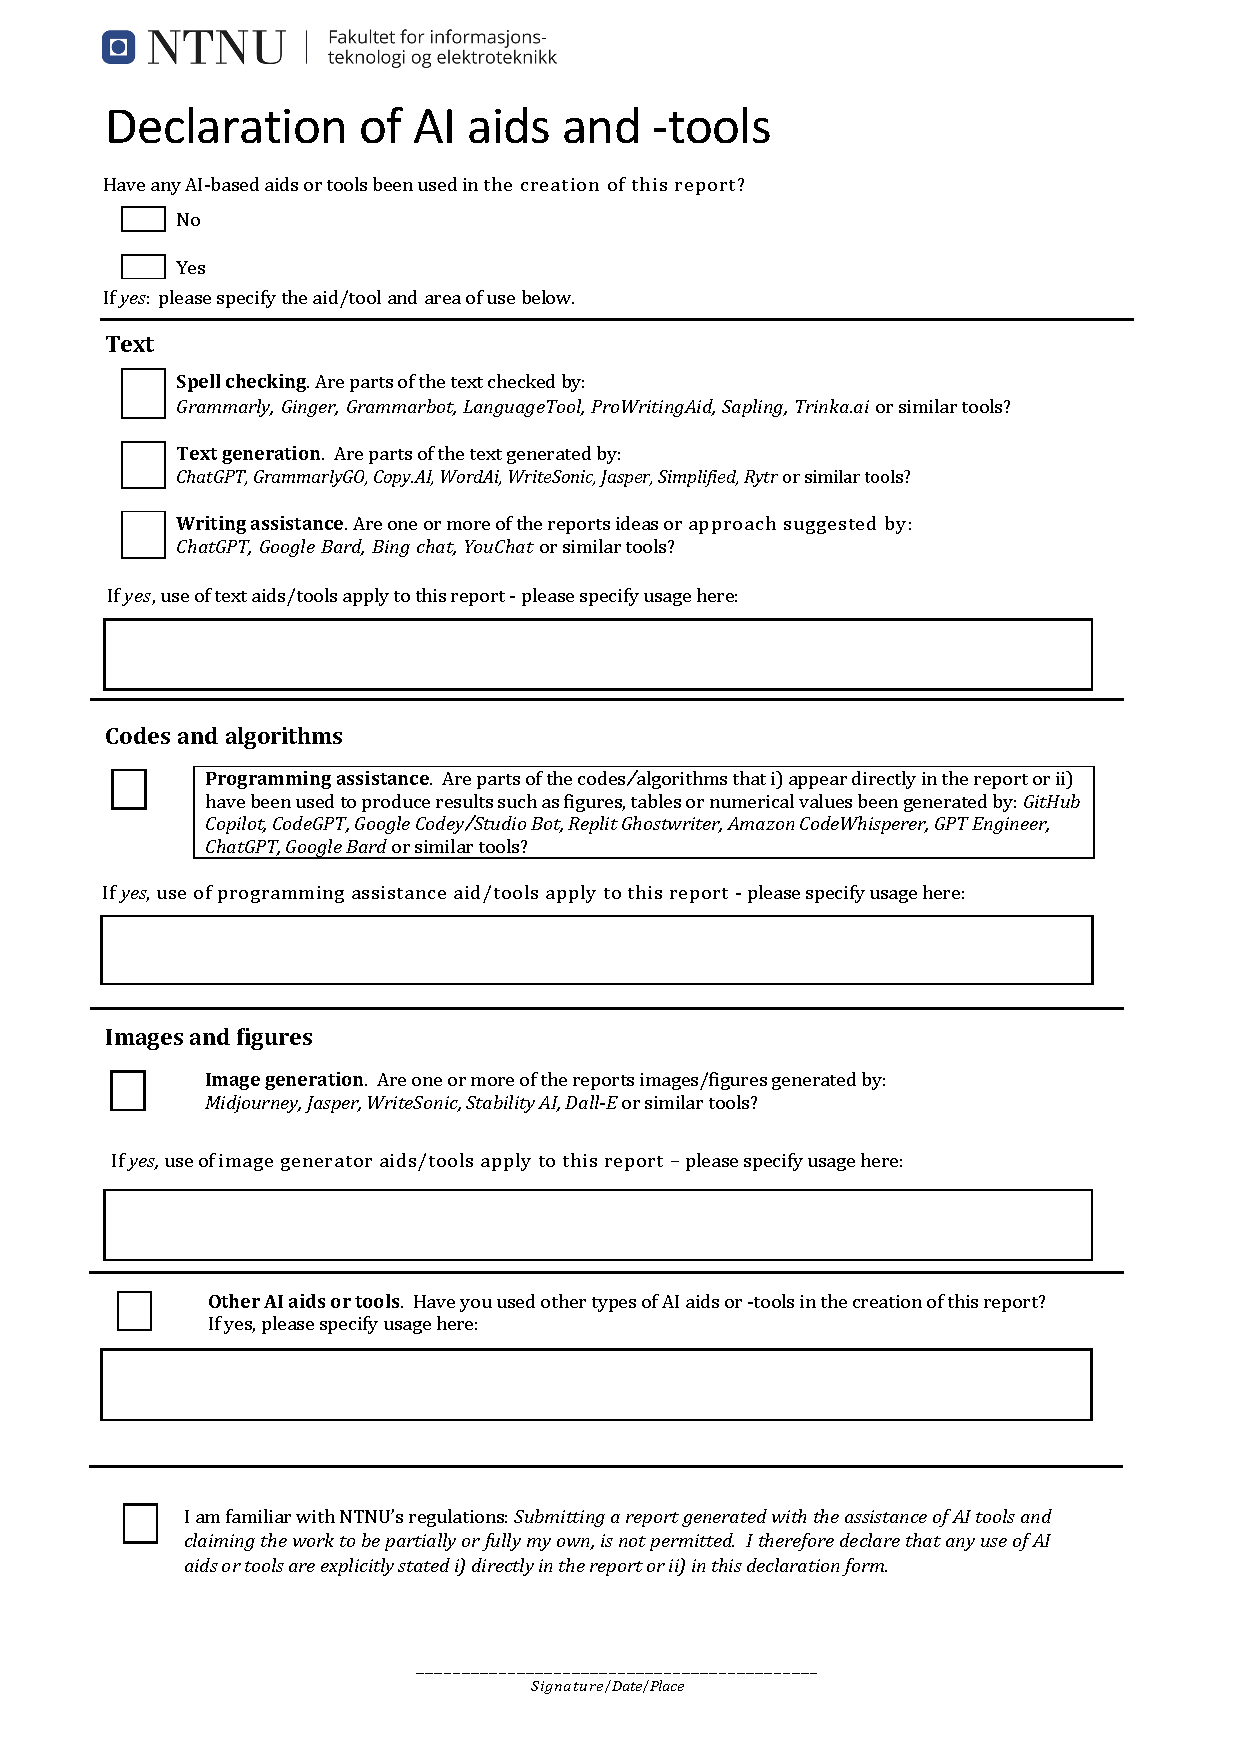
\includepdf[pages=-]{AI_declaration.pdf}


\chapter*{Abstract}

This project develops a numerical method for identifying multiple simultaneous leaks in a single pipeline, where leak identification refers to both localization and size estimation. The method relies solely on steady-state inlet and outlet head and flow measurements to support software-based leak identification in water distribution systems with limited monitoring equipment. Pipeline leakage causes substantial water loss, increased operational costs, and infrastructure risk, making practical methods for leak identification important. However, existing steady-state methods are largely limited to one or two leaks, while methods for several leaks typically require transient data or additional sensors.\\

To address this gap, the leak identification problem was formulated as a nonlinear residual problem and solved using a Levenberg--Marquardt method with an analytically derived Jacobian. The method was evaluated through an extensive simulated test framework and on published simulated two-leak experiments. The results show that the method performs reliably for two and three leaks and can still provide useful localization for four leaks in many cases. A condition number analysis further showed that the inverse problem becomes rapidly more ill-conditioned as the number of leaks increases. Combined with the empirical results, this suggests that identifying five or more simultaneous leaks is likely close to the upper limit of what is numerically feasible using only steady-state endpoint measurements.\\

These findings show that steady-state endpoint measurements can identify more simultaneous leaks than comparable published steady-state methods. At the same time, they reveal a practical limit imposed by the intrinsic conditioning of the inverse problem.
\chapter*{Sammendrag}

Dette prosjektet utvikler en numerisk metode for å identifisere flere samtidige lekkasjer i et rør, der lekkasjeidentifikasjon omfatter både lokalisering og estimering av lekkasjestørrelse. Metoden bygger utelukkende på stasjonære målinger av trykkhøyde og vannføring ved innløp og utløp og er ment å støtte programvarebasert lekkasjeidentifikasjon i vannforsyningssystemer med begrenset måleutstyr. Lekkasjer i rørledninger fører til betydelige vanntap, økte driftskostnader og økt risiko for infrastrukturen, noe som gjør praktiske metoder for lekkasjeidentifikasjon viktige. Eksisterende stasjonære metoder er imidlertid i stor grad begrenset til én eller to lekkasjer, mens metoder for flere lekkasjer vanligvis krever transiente data eller ekstra sensorer.\\

For å håndtere dette gapet ble lekkasjeidentifikasjonsproblemet formulert som et ulineært residualproblem og løst ved hjelp av en Levenberg--Marquardt-metode med en analytisk utledet Jakobimatrise. Metoden ble evaluert gjennom et omfattende simulert testrammeverk og mot publiserte simulerte eksperimenter med to lekkasjer. Resultatene viser at metoden fungerer pålitelig for to og tre lekkasjer og at den i mange tilfeller fortsatt kan gi nyttig lokalisering for fire lekkasjer. En kondisjonstallsanalyse viste videre at det inverse problemet raskt blir dårligere kondisjonert når antall lekkasjer øker. Sammen med de empiriske resultatene tyder dette på at identifisering av fem eller flere samtidige lekkasjer trolig ligger nær den øvre grensen for hva som er numerisk gjennomførbart ved bruk av kun stasjonære endepunktsmålinger.\\

Funnene viser at stasjonære endepunktsmålinger kan identifisere flere samtidige lekkasjer enn sammenlignbare publiserte stasjonære metoder. Samtidig avdekker de en praktisk grense som skyldes den iboende kondisjoneringen til det inverse problemet.
\chapter*{Preface}

This report marks the completion of my five years at Norwegian University of Science and Technology (NTNU) and represents my final work toward a Master’s degree in Cybernetics and Robotics. The thesis was written as part of the course TTK4900 Engineering Cybernetics, Master’s Thesis, at the Department of Engineering Cybernetics, and constitutes 30 credit points.\\

The thesis has been carried out independently, with guidance and valuable feedback from my supervisor, Prof. Ole Morten Aamo. I would like to express my sincere gratitude for his support, discussions, and supervision throughout the project.\\

At the beginning of this project, it was a great surprise to learn about the extent of leakage in water distribution networks worldwide, and especially how significant the problem is in Norway. Water leakage poses both economic and environmental challenges, and I hope the work presented in this thesis will contribute to more efficient maintenance and repair of damaged water infrastructure.


\tableofcontents

\cleardoublepage
\phantomsection
\addcontentsline{toc}{chapter}{\listfigurename}
\listoffigures

\cleardoublepage
\phantomsection
\addcontentsline{toc}{chapter}{\listtablename}
\listoftables

\cleardoublepage
\phantomsection
\addcontentsline{toc}{chapter}{\listalgorithmcfname}
\listofalgorithms

\chapter*{\glossaryname}
\addcontentsline{toc}{chapter}{\glossaryname}
{
\renewcommand{\arraystretch}{1.5}
\printnoidxglossary[sort=use]
}

\chapter{Introduction}

\section{Motivation and Background}

Leakage in water distribution systems is a major global problem with economic, environmental, and operational consequences. Estimates from the World Bank show that developing countries lose tens of millions of cubic meters of treated water each day due to pipe leakage. This volume could otherwise supply a large population \cite{kingdom2006}.\\

\begin{figure}[h!]
    \centering
    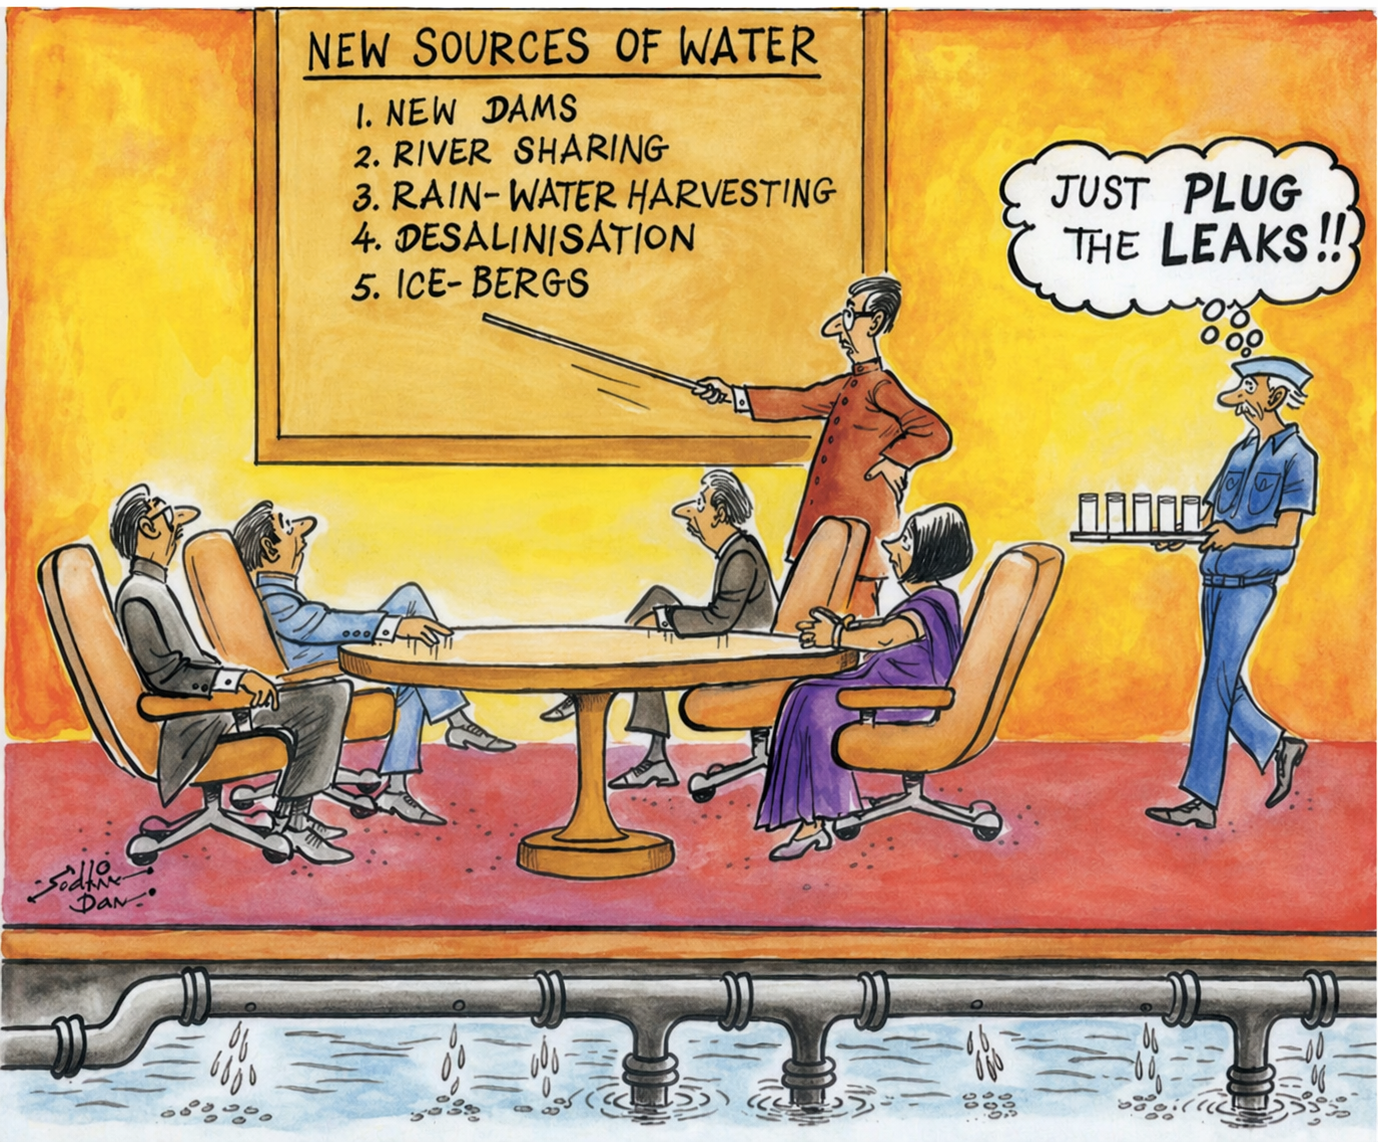
\includegraphics[width=0.6\linewidth]{images/plug_the_leaks.png}
    \caption{Illustration from the Water and Sanitation Program of the World Bank \cite{iwa2007} (Quality enhanced by ChatGPT) }
    \label{fig:plug_the_leaks}
\end{figure}

These losses are often described as non-revenue water (NRW), which refers to the difference between the volume of water entering the distribution system and the volume billed to consumers. NRW includes physical losses caused by leakage as well as other forms of water that do not generate revenue. Recent global estimates indicate that NRW amounts to approximately 346 million $m^3$/day, or 126 billion $m^3$/year, which equates to 30\% of all distributed water worldwide, with an annual cost of around USD 39 billion \cite{liemberger2018}. Pipe leaks may also damage surrounding infrastructure and pose environmental and public health risks \cite{qi2018}. Leaks may reverse the flow direction, potentially causing water quality issues, and significantly increase flow velocities, which can dislodge biofilms and further deteriorate water quality. \\

Leakage levels vary significantly between countries. In Norway, water distribution systems experience some of the highest leakage rates in Europe. The average water loss is around 30\%, and in several systems, more than 40\% of treated drinking water is lost due to leakage in the network \cite{norskvann2026}.\\

Leak detection and repair are often difficult and expensive in practice. Many leaks occur underground and may remain undetected for long periods, especially when water does not reach the surface. Once a leak is suspected, utilities often rely on field inspections, acoustic surveys, and other local investigations to estimate its location before excavation begins \cite{hu2021}. This process requires significant time and cost because excavation is disruptive, and the exact leak location often remains uncertain until digging begins. This limitation has increased interest in software-based and data-driven detection and localization methods.\\

Specifically, there is a practical interest in identification methods that rely only on head and flow measurements. These variables are commonly measured in real pipeline systems, which makes them suitable for practical monitoring applications \cite{hu2021}. Available sensors do not always sample at a sufficiently high frequency to detect hydraulic transients, which may occur over very short time scales. In such cases, steady-state information provides a more reliable basis for analysis. This makes methods based on steady-state inlet and outlet measurements of head and flow relevant to investigate.\\

The detection and localization of multiple simultaneous leaks has received limited attention in the literature. It is pointed out in \cite{torres2024} that truly simultaneous leak events are generally considered unlikely. Despite this, the problem remains relevant in practice. In older water networks that have not been continuously monitored, multiple defects may already be present by the time sensors are installed, and measurements are collected. Based on the available hydraulic data, this situation is equivalent to observing multiple concurrent leaks. This provides clear motivation to investigate whether several leaks can be identified in pipe segments between available measurement points.

\newpage
\section{Master's Thesis Assignment}

This section outlines the master's thesis assignment. It begins with a description of the task, followed by the delimitations that set the scope of the work. Finally, there is a brief discussion of the work's relevance to sustainability.

\subsection{Task Description} \label{sec:task_desc}

Consider a pipe of length \gls{ell}, where \gls{z} $\in [0, \ell]$ denotes position along the pipe. Assume steady-state operation, and let
\[
q : [0,\ell] \to \mathbb{R}_{\geq0}, \qquad h : [0,\ell] \to \mathbb{R}_{\geq0}
\]
denote the volumetric discharge and piezometric head (from now regarded as flow and head for brevity). Thus, \gls{qz} and \gls{hz} represent the flow and head at position \gls{z}, which are both assumed strictly positive along the pipe. Suppose \gls{n} leaks occur at locations
\[
0 < z_1 < \dots < z_n < \ell,
\]
with corresponding leak discharges $\tilde q_1,\dots,\tilde q_n$, where \gls{tildeqi} and \gls{zi} correspond to the $i$-th leak. Assuming small leak openings, each leak is modeled as a valve by
\[
\tilde{q}_i = c_i \sqrt{h(z_i)},
\]
where \gls{ci} $>0$ is a constant discharge coefficient characterizing the $i$-th leak. 
The steady-state head loss along the pipe is governed by
\begin{equation}
\label{eq:task_desc_ufunc}
\frac{dh}{dz} = -U(q(z)),
\end{equation}
where \gls{U} $:[0,\infty)\to[0,\infty)$ is smooth and strictly increasing. For notation purposes, let the flow and head at the inlet and outlet be defined by
\[
\text{\gls{q0}} := q(0), \qquad \text{\gls{ql}} := q(\ell), \qquad
\text{\gls{h0}} := h(0), \qquad \text{\gls{hl}} := h(\ell).
\]
Since flow is conserved between leak locations, $q$ is piecewise constant. Introducing $z_0:=0$ and $z_{n+1}:=\ell$, the flow is given by
\[
q(z)=\text{\gls{qi}}:=
\begin{cases}
q_0, & \text{for } z \in [0, z_1), \quad i = 0, \\[6pt]
q_0 - \sum_{k=1}^{i} \tilde{q}_k, & \text{for } z \in [z_i, z_{i+1}), \quad i = 1, \dots, n,
\end{cases}
\]
where also $q_n=q_{\ell}$ for notation consistency. From \cref{eq:task_desc_ufunc}, it follows that the head is continuous and piecewise linear along the pipe. Let
\[
L_{i+1} := z_{i+1}-z_{i},
\qquad i=0,\dots,n,
\]
denote the lengths of the non-leaking segments, so that
\[
\sum_{i=1}^{n+1} \text{\gls{Li}} = \ell.
\]
The head at the $i$-th leak location is denoted by
\[
\text{\gls{hi}} := h(z_i), \qquad i=1,\dots,n,
\]
and for notation consistency, let $h_{n+1}:=h_{\ell}$. The notation for a pipe is illustrated in \autoref{fig:leak_notation}.\\

\begin{figure}[h!]
    \centering
    \input{figures/tikz_pipe}
    \caption{Notation used for a pipe with $n$ leaks.}
    \label{fig:leak_notation}
\end{figure}

Suppose the flow and head at the pipe's inlet and outlet can be measured at \gls{m} different steady-state operating points. For the $j$-th operating point, let
\[
\text{\gls{y0}} :=\begin{bmatrix}
    h_0^{(j)} \\[0.4em]
    q_0^{(j)}
\end{bmatrix}, \quad
\text{\gls{yl}} := \begin{bmatrix}
    h_{\ell}^{(j)} \\[0.4em]
    q_{\ell}^{(j)}
\end{bmatrix}, \quad
j=1,\dots,m,
\]
define the vectors of inlet and outlet measurements. The complete matrices of inlet and outlet measurements are defined by
\[
\text{\gls{M0}}
:=
\begin{bmatrix}
y_0^{(1)} & \cdots & y_0^{(m)}
\end{bmatrix} \in\mathbb{R}^{2\times m},
\qquad
\text{\gls{Ml}}
:=
\begin{bmatrix}
y_{\ell}^{(1)} & \cdots & y_{\ell}^{(m)}
\end{bmatrix} \in\mathbb{R}^{2\times m}.
\]
For notation purposes, let all measurements be defined by
\[
\text{\gls{M}}
:=
\begin{bmatrix}
\mathcal{M}_0 \\[0.4em] 
\mathcal{M}_{\ell}
\end{bmatrix} \in\mathbb{R}^{4\times m} 
\]
and \gls{y} $:=\begin{bmatrix}
    \text{\gls{y0}} \\[0.4em]
    \text{\gls{yl}}
\end{bmatrix} \in \mathbb{R}^4$ is defined as the $j$-th column of \gls{M}.\\

\begin{definition}{Leak Identification Problem}{leak-identification}
For some leak parameters $\vartheta := \begin{bmatrix}
    z_1 & \cdots & z_n & c_1 & \cdots & c_n
\end{bmatrix}^\top$, assume there exists a function
\[
\mathcal{F}_{\mathcal{M}_0}(\vartheta) = \mathcal{M}_\ell,
\]
parametrized by some fixed inlet measurements \gls{M0}, which produces the outlet measurements \gls{Ml}. The leak identification problem is the inverse problem of recovering leak parameters $\vartheta$ from \gls{M0} and \gls{Ml}:
\[
\vartheta = \mathcal{F}_{\mathcal{M}_0}^{\,-1}(\mathcal{M}_\ell)
\]
\end{definition}

\begin{definition}{Leak Identification Problem (alt)}{leak-identification2}
Let the input-output relation of a pipe with $n$ leaks be defined by
\begin{equation*}
    \mathcal{P}_n(\vartheta) : \mathcal{M}_0 \mapsto \mathcal{M}_\ell,
\end{equation*}
where $\vartheta := \begin{bmatrix}
    z_1 & \cdots & z_n & c_1 & \cdots & c_n
\end{bmatrix}^\top$ denotes the leak parameters.\\

The leak identification problem is to identify a parameter vector $\vartheta$ that is consistent with the observed input-output behavior
given by $\mathcal{M}_0$ and $\mathcal{M}_\ell$.
\end{definition}

\begin{samepage}
The following tasks should be performed:
\begin{enumerate}
    \item Literature review (see \cite{peralta2023}, \cite{molno2024parallel}, \cite{molno2024conditions} for a starting point). \\

    \item Assuming that the function \gls{U}, the number of leaks \gls{n}, and the pipe length \gls{ell} are known, develop and implement a method for solving the leak identification problem as defined in \autoref{def:leak-identification}.\\

    % \item Assuming that the function \gls{U}, the number of leaks \gls{n}, and the pipe length \gls{ell} are known, develop and implement a method for identifying the leak locations $(z_1,\dots,z_n)$ and the corresponding discharge coefficients $(c_1,\dots,c_n)$ from the measurement collection \gls{M}, consisting solely of inlet and outlet measurements obtained from \gls{m} different steady-state operating points.\\

    \item Investigate the maximum number of leaks feasible to identify.\\
    
    \item Perform simulated tests to investigate the performance of the method in the idealized setup (\gls{U}, \gls{n}, and \gls{ell} are known).\\

    \item Investigate how the method performs when parameters are uncertain, or noise is introduced to measurements.\\
\end{enumerate}
\end{samepage}

\newpage
\subsection{Delimitations}

The following delimitations restrict the scope of the work:

\begin{itemize}

\item \textbf{Leak detection:}
The problem of detecting leaks is not addressed. Under the adopted assumptions, the presence of a leak is trivial, since a discrepancy between the inlet and outlet flow indicates leakage. References such as \cite{isermann1997} and \cite{blanke2006} describe detection methods and alarm systems in detail.\\

\item \textbf{Number of leaks:}
The case of a single leak ($n = 1$) is not considered, since this problem is well defined and can be solved analytically. It is treated as trivial in this context. The thesis focuses on multiple simultaneous leaks ($n \geq 2$).\\

\item \textbf{System scope:}
The system consists of a single pipeline segment. Pipe networks with branches or junctions are not considered.\\

\item \textbf{Model assumptions:}
To simplify the derivations, the hydraulic resistance function will be limited to the quadratic form (based on the derivation in \autoref{chap:model})
\[ U(q(z)) = \theta q^2(z), \]
where \gls{theta} is assumed to be a known and constant friction parameter. It should be noted that these assumptions are not required by the method, and more advanced friction models, or parameters as functions of $z$, could be incorporated.\\

Leaks are assumed to be small relative to the total flow. This ensures that flow and head are non-zero at the outlet. The flow is assumed unidirectional along the pipe, with leaks limited only to outward flow and no external inflow.\\

Only steady-state conditions are considered. Transient effects such as pressure waves and time-dependent flow dynamics are excluded.\\

The main analysis follows idealized conditions, without modeling or measurement errors, and assumes the number of leaks is known. The aim is to isolate the problem's fundamental theoretical properties and limitations. This provides insight into the underlying challenges that remain relevant under non-ideal assumptions, since the limitations present in the ideal case also constrain more realistic and complex scenarios.\\

For completeness, a brief extension in \autoref{sec:n_not_known} considers the case where the number of leaks is unknown, and \autoref{sec:mod_err} examines the impact of model and measurement errors. For space reasons, only modeling errors in \gls{theta} are considered, since it is assumed to be the most difficult parameter to estimate in practice.\\

\item \textbf{Measurements:}
In a practical situation, \gls{M} would come from measuring a physical system operating at different steady-states. Due to data availability and the scope of the problem, $\mathcal{M}$ will be generated in this work through simulation, where the pipe parameters \gls{ell} and \gls{theta} are known exactly. The measurements are therefore free of both model error and measurement noise.\\

\end{itemize}

\subsection{Sustainability Relevance}

This work relates to sustainability by reducing water losses and improving resource efficiency in water distribution systems. Lower leakage rates reduce unnecessary water extraction and the energy required for treatment and pumping, thereby decreasing the overall environmental footprint of water supply operations.\\

These aspects are linked to several of the United Nations Sustainable Development Goals \cite{un_goals}. In particular, the work supports SDG 6 (Clean Water and Sanitation) by improving water-use efficiency and SDG 9 (Industry, Innovation and Infrastructure) by developing enhanced monitoring and diagnostic methods. It also contributes to SDG 12 (Responsible Consumption and Production) by promoting more efficient resource use and reducing waste.

\section{Overall Organization of Work}

The project combined method development, numerical testing, and mathematical analysis of the underlying problem structure. The work was primarily theoretical, with additional focus on practical implementation and applicability to real-world problems. The main objective was to develop a program capable of solving the leak identification problem defined in \autoref{def:leak-identification}. The developed framework was evaluated using simulated data, where performance was assessed through empirical results.\\

The work presented in this thesis was initiated independently for the project and was not based on existing implementations, previously collected datasets, or prior development work. The initial stages of the project, therefore, focused on establishing the theoretical framework and developing the associated software tools from first principles.\\

An extensive literature review was conducted before and during the development process. Alongside traditional academic search engines, the large language model, ChatGPT \cite{chatgpt}, supported the literature search process. Detailed descriptions of research topics and information needs were provided to the model to identify potentially relevant publications. This approach made it possible to find relevant work and conceptual connections even when suitable terminology was unknown or difficult to express through standard keyword searches. Previous studies have shown that such models can support literature search and screening tasks within scientific domains \cite{jin2024pubmedandbeyond}, \cite{dennstadt2024titleandabstract}, \cite{delgado-chaves2025transforming}. The identified papers were then studied in detail, and their references were used to further expand the review. Google Scholar and arXiv were used to access specific publications, while Connected Papers \cite{connectedpapers} was used to improve the coverage of related work within the field.\\

To support the software development process, AI-assisted programming tools such as Codex \cite{codex} and Cursor \cite{cursor} were used for rapid prototyping and agent-based debugging. These tools enabled efficient testing of ideas and accelerated the development process. For numerical simulations, NTNU provided access to dedicated computing resources, enabling computationally demanding workloads to be executed in parallel. The total simulation time is estimated to be approximately 200 hours.\\

Throughout the writing process, ChatGPT was used to reformulate draft text, format mathematical expressions, and assist with implementing TikZ figures. Grammarly \cite{grammarly} has been used throughout the writing of this report for spell checking, improving sentence structure, and rewording. Additional details regarding the use of AI tools are provided in the attached AI declaration.

\newpage
\section{Structure of the Report}

\renewcommand{\descriptionlabel}[1]{\normalfont #1}
\begin{description}[itemsep=2pt, topsep=0pt, parsep=0pt]
    \item[Chapter 1] presents the motivation for the work, defines the assignment, and describes the organization of the project.

    \item[Chapter 2] gives an overview of the studied literature and an analysis of relevant published methods.

    \item[Chapter 3] introduces the theoretical background for nonlinear residual problems and optimization methods, providing the essential knowledge needed to follow the methods and algorithms developed.

    \item[Chapter 4] derives the mathematical model for a water pipe with leaks used in this work.

    \item[Chapter 5] presents how the problem is formulated as a nonlinear residual problem and proposes a solver design to find a solution. 

    \item[Chapter 6] performs a mathematical analysis of the residual function to investigate two things. First is how the measurements affect the solution space, and how different steady-state operating points can be chosen to improve the identifiability of the leaks. Secondly, how the increase in the number of leaks affects the feasibility of identifying them. 

    \item[Chapter 7] compares the proposed method against a published method and further tests it using an extensive test framework, yielding empirical results on the method's performance. The chapter also presents how the method performs when the number of leaks is unknown and when it is introduced to model and measurement errors.

    \item[Chapter 8] discusses the method's limitations based on the results, how the method can be useful in practice, and future work. 

    \item[Chapter 9] concludes the report by summarizing the contributions and achievements.
\end{description}


% \input{chapters/2-literature}
% \chapter{Theory}
\label{chap:theory}
\section{Nonlinear Residual Problems}

Let 
\[
r : \mathbb{R}^n \to \mathbb{R}^m
\]
be a nonlinear and continuously differentiable function. The nonlinear residual problem is to find any
\begin{equation*}
     x^\ast \in \mathbb{R}^n \quad \text{such that} \quad r(x^*) = 0.
\end{equation*}
The function $r(x)$ is referred to as the \emph{residual} function.

\subsection{The Jacobian Matrix}

The Jacobian of \(r\) at a point \(x \in \mathbb{R}^n\) is the matrix
\[
J(x) = \frac{\partial r(x)}{\partial x}
=
\begin{bmatrix}
\dfrac{\partial r_1}{\partial x_1} & \cdots & \dfrac{\partial r_1}{\partial x_n} \\
\vdots & \ddots & \vdots \\
\dfrac{\partial r_m}{\partial x_1} & \cdots & \dfrac{\partial r_m}{\partial x_n}
\end{bmatrix}
\in \mathbb{R}^{m \times n}.
\]

Using first-order Taylor expansion, the Jacobian represents the first-order linearization of \(r\) near \(x\):
\begin{equation}
\label{eq:jac_res_approx}    
r(x + \Delta x) \approx r(x) + J(x)\,\Delta x.
\end{equation}

Thus, \(J(x)\) describes the local sensitivity of the residual with respect to perturbations in the variables.

\subsection{Existence and Number of Local Solutions}
\label{sec:sol_existence}

Let $x^\ast \in \mathbb{R}^n$ satisfy $r(x^\ast)=0$, and assume that $r$ is continuously differentiable in a neighborhood of $x^\ast$.
Then it follows from the Implicit Function Theorem that the local structure of solutions is determined by the rank of the Jacobian $J(x^\ast)$, provided the rank is constant in a neighborhood of $x^\ast$.

\paragraph{Case $m = n$ (square system).}

Suppose $m=n$ and let $x^\ast$ satisfy $r(x^\ast)=0$.  
If the Jacobian $J(x^\ast)$ is nonsingular,
\[
\det J(x^\ast) \neq 0,
\]
then, by the Implicit Function Theorem, $x^\ast$ is a locally unique solution. In particular, there exists a neighborhood around $x^\ast$ in which no other solutions exist.

If $J(x^\ast)$ is singular, the local behavior of the solution set cannot be determined from first-order information alone. In this case, the solution may fail to be isolated, and additional solutions may exist arbitrarily close to $x^\ast$.

\paragraph{Case $m < n$ (underdetermined system).}

If $J(x^\ast)$ has full row rank $m$, then the solution set near $x^\ast$ is not isolated. Instead, it forms a smooth manifold of dimension $n - m$.
Hence, there are infinitely many nearby solutions, parameterized by $n-m$ degrees of freedom.

\paragraph{Case $m > n$ (overdetermined system).}

In an overdetermined system, the number of equations exceeds the number of unknowns, so the system generally has no exact solution.
Suppose, however, that a point $x^\ast$ satisfies $r(x^\ast)=0$.
If $J(x^\ast)$ has full rank $n$, the constraints are locally independent and restrict all directions in $\mathbb{R}^n$, so the solution $x^\ast$ is locally isolated.
If $\operatorname{rank} J(x^\ast)<n$, the constraints are not independent, and the solution is structurally unstable under perturbations of $r$.

\paragraph{Global Solution.}

The Jacobian $J(x^\ast)$ characterizes only the \emph{local} structure of the solution set. Even if $J(x^\ast)$ is nonsingular and $x^\ast$ is locally unique, the nonlinear system may possess additional solutions elsewhere in $\mathbb{R}^n$. Consequently, local invertibility of the Jacobian does not imply global uniqueness.

Global existence or uniqueness of a solution to $r(x)=0$ requires additional structural assumptions on $r$, such as global injectivity or strong monotonicity. In the absence of such global properties, the existence and uniqueness of a solution cannot be guaranteed from an analysis of the Jacobian.

\section{Local Sensitivity of the Residual}

The Jacobian matrix characterizes how perturbations in the variables influence the residual locally (\cref{eq:jac_res_approx}). The magnitude of this influence may vary significantly depending on the direction of perturbation. Understanding these directional effects is important for assessing how reliably the variables can be inferred from the residual.\\

Local sensitivity can be analyzed through the singular values of the Jacobian, which quantify how strongly perturbations in different directions affect the residual.

\subsection{Singular Value Decomposition}

Let $J \in \mathbb{R}^{m \times n}$ denote the Jacobian evaluated at a point of interest. The singular value decomposition (SVD) of $J$ is given by
\begin{equation*}
J = U \Sigma V^\top,
\end{equation*}
where

\begin{itemize}
\item $U \in \mathbb{R}^{m \times m}$ and $V \in \mathbb{R}^{n \times n}$ are orthogonal matrices,
\item $\Sigma \in \mathbb{R}^{m \times n}$ is diagonal,
\item the diagonal entries satisfy
\[
\sigma_1 \ge \sigma_2 \ge \dots \ge \sigma_p \ge 0,
\]
with $p = \min(m,n)$.
\end{itemize}

The singular values describe how perturbations in specific directions of the variable space influence the residual. The columns of $V$ define orthogonal directions in $\mathbb{R}^n$, while the corresponding singular values determine the magnitude of the resulting change in the residual.\\

Large singular values correspond to directions in which small perturbations of the variables produce relatively large changes in the residual. Conversely, small singular values correspond to directions in which the residual changes only weakly. If one or more singular values are close to zero, the Jacobian is nearly rank-deficient, indicating directions along which the residual provides little local information about the variables.

\subsection{Condition Number of the Jacobian}

A scalar measure of local sensitivity is given by the condition number of the Jacobian,
\begin{equation}
    \label{eq:cond_num_def}
\kappa(J) = \frac{\sigma_1}{\sigma_p},
\end{equation}
where $\sigma_1$ and $\sigma_p$ denote the largest and smallest singular values of $J$, respectively.\\

The condition number measures how differently perturbations in various directions affect the residual. If the singular values are of comparable magnitude, perturbations in different directions produce changes in the residual of similar size, indicating balanced local sensitivity.\\

If the smallest singular value is much smaller than the largest, some directions produce much weaker changes in the residual than others. In such situations, small perturbations in the residual may correspond to large changes in the variables, indicating reduced numerical stability.\\

If $\sigma_p = 0$, the Jacobian is rank-deficient and the condition number is infinite. In this case, there exist directions in which perturbations of the variables do not influence the residual to first order.

\section{Optimization Methods}
\label{sec:theory_optmet}

In practice, it is often hard to solve a nonlinear residual problem directly. Instead, the problem can be reformulated as a nonlinear least squares optimization problem with the scalar objective function
\begin{equation}
f(x) = \frac{1}{2} \| r(x) \|^2 \in \mathbb{R}.
\label{eq:least_squares_objective}
\end{equation}
Solving the minimization problem,
\begin{equation}
\label{eq:min_problem}
    x^\ast = \underset{x}{\text{argmin}} \ f(x) = \underset{x}{\text{argmin}} \ \frac{1}{2} \| r(x) \|^2,
\end{equation}
satisfies $r(x^*) = 0$ if an exact solution exists. If no exact solution exists, or if the system is overdetermined, the formulation yields a solution that minimizes the residual norm.\\

Solving \cref{eq:min_problem} is very hard to solve in general \cite{madsen2004}, since there might exist local minima that are larger than a global minima. \cite{nielsen1999}

A group of methods used to solve the optimization problem operates by iteratively evaluating the objective function at the current iterate $x_k$ and determining a step $s_k$ that decreases the cost function. The next iterate is computed as
\begin{equation}
\label{eq:step_update_rule}
    x_{k+1} = x_k + s_k,
\end{equation}
with the goal of choosing $s_k$ so that
\begin{equation*}
    f(x_{k+1}) < f(x_k).
\end{equation*}
There are two main frameworks for controlling how the step $s_k$ is chosen, called \textit{Line Search} and \textit{Trust Region} methods. This section will introduce these frameworks along with common algorithms used to solve the minimization problem.

\subsection{Line Search Methods}
\begin{equation}
    s_k = \alpha_k p_k
\end{equation}
\begin{itemize}
    \item Armijo Backtracking\\
    \item Wolfe Conditions
\end{itemize}

\subsection{Gradient Descent}
Gradient descent is a simple method that is based on moving in the direction of the negative gradient of the objective function. 
Using the chain rule, the gradient of $f$ is given by
\begin{equation}
\label{eq:gradient_f}
    \nabla f(x) = J(x)^\top r(x),
\end{equation}
where $J(x)$ denotes the Jacobian of the residual function.

At the current iterate $x_k$, the search direction is chosen as the direction of steepest descent:
\begin{equation}
\label{eq:steepest_descent}
    p_k = - \nabla f(x_k) = - J(x_k)^\top r(x_k).
\end{equation}

Gradient descent is simple to implement and requires only first-order derivative information through the Jacobian. It is computationally inexpensive per iteration and applicable even when second-order derivatives are unavailable. However, the method may converge slowly, especially for ill-conditioned problems or narrow curved valleys in the objective function. Its performance is sensitive to scaling and may require many iterations to achieve high accuracy.

\subsection{Newton's Method}

Newton's method incorporates second-order information of the objective function. 
The gradient of $f$ is given by \cref{eq:gradient_f} and the Hessian is given by
\begin{equation}
\label{eq:hessian}
    \nabla^2 f(x) = J(x)^\top J(x) + \sum_{i=1}^m r_i(x)\nabla^2 r_i(x).
\end{equation}

At iteration $k$, the Newton search direction is obtained by solving the linear system
\begin{equation*}
    \nabla^2 f(x_k) p_k = - \nabla f(x_k).
\end{equation*}

By incorporating curvature information, Newton's method typically achieves quadratic convergence in a neighborhood of a solution, provided that the Hessian is nonsingular. This represents a significant improvement over gradient descent in terms of local convergence speed.

However, the method requires computation and factorization of the Hessian matrix, which can be expensive for large-scale problems. Moreover, if the Hessian is indefinite or poorly conditioned, the method may fail to produce a descent direction without additional safeguards.

\subsection{Gauss--Newton Method}

The Gauss--Newton method is tailored specifically to nonlinear least squares problems. 
It is based on an approximation of \cref{eq:hessian},
\begin{equation*}
    \nabla^2 f(x) \simeq J(x)^\top J(x),
\end{equation*}
which neglects the second-order term involving $\nabla^2 r_i(x)$.

The search direction is therefore computed by solving
\begin{equation}
\label{eq:gauss_newton}
    J(x_k)^\top J(x_k) p_k = - J(x_k)^\top r(x_k).
\end{equation}

This approximation avoids explicit computation of second derivatives and reduces computational cost compared to full Newton's method. When the residual is small near the solution, the neglected term becomes insignificant, and the method exhibits fast local convergence.

The Gauss--Newton method may perform poorly when the residual is large or when $J(x_k)^\top J(x_k)$ is rank deficient. In such cases, the approximation of the Hessian can be inaccurate, and additional regularization techniques may be required to ensure robustness.

\subsection{Trust Region Methods}
\label{sec:trust_region_methods}

Trust region methods determine the step $s_k$\footnote{The step $s_k$ is the same as the search direction $p_k$ with $\alpha=1$.} by minimizing a local model of the objective function within a restricted neighborhood around the current iterate. From \cite{madsen2004}, a typical model is the second order taylor expansion, using the Gauss--Newton approximation of the Hessian, 
\begin{equation}
\label{eq:mk}
f(x_k+s) \simeq m_k(s) = f(x_k) + r(x_k)^\top J(x_k) \, s + \frac{1}{2} s^\top J(x_k)^\top J(x_k) \, s
\end{equation}

In the trust region method, it is assumed that there exists a radius $\Delta$ around $x_k$, such that the model $m_k(s)$ is sufficiently accurate within the region. The step is then computed by solving the constrained minimization problem,

\begin{equation}
\label{eq:trust_region_subproblem}
    s_k = \underset{s}{\text{argmin}} \ m_k(s) \quad \text{subject to} \quad \|s\| \leq \Delta_k.
\end{equation}

In practice, this is solved through solving a damped problem, where the step is computed by solving the unconstrained minimization problem,
\begin{equation}
\label{eq:damped_problem}
    s_k = \underset{s}{\text{argmin}} \ \left(m_k(s) + \frac{1}{2} \ \lambda \ s^\top s\right),
\end{equation}
where $\lambda \geq 0$ is the damping parameter, and $\lambda \ s^\top s$ penalizes large steps. 

For a given $\Delta$ or $\lambda$, if no sufficient step $s_k$ is found such that $f(x_k+s_k)<f(x_k)$ (assuming $x_k$ is not a solution), the parameters ($\Delta,\lambda$) must be tuned such that a sufficient step is found. Since $m_k(s)$ is assumed to be a sufficient approximation for $f(x_k+s)$ when $s$ is sufficiently small, the trust region should be decreased ($\lambda$ increased) for the next iteration. When a sufficient step is found, it indicates that $m_k(s)$ is a good approximation, and the trust region can be increased ($\lambda$ decreased), aiming for faster convergence.

\subsection{Levenberg--Marquardt Method} \label{sec:levenberg_marquardt}

The Levenberg--Marquardt (LM) method is a damped Gauss--Newton method designed for solving nonlinear least--squares problems. It can be interpreted as a trust region method where the step is computed from a regularized Gauss--Newton system. The damping parameter, $\lambda$, controls the transition between the Gauss--Newton and steepest descent method.

At iteration $k$, the LM step is obtained by solving the linear system
\begin{equation} \label{eq:lm_system}
    \left( J(x_k)^\top J(x_k) + \lambda I \right) s_k
    =
    - J(x_k)^\top r(x_k),
\end{equation}
As $\lambda \to 0$, the system approaches the Gauss--Newton equations, \cref{eq:gauss_newton}. For large $\lambda$, the step approaches,
\begin{equation*}
    s_k \simeq -\frac{1}{\lambda}J(x_k)^\top r(x_k),
\end{equation*}
which is the steepest descent direciton, \cref{eq:steepest_descent}, with a small step lenght, $\alpha=\lambda^{-1}$.

The damping parameter must be initialized before the iterations begin. \cite{nielsen1999} states that the initial value should relate to the magnitude of the eigenvalues, and proposes
\begin{equation} \label{eq:init_lambda}
\lambda_0 = \tau \max \left( \operatorname{diag}(J(x_0)^\top J(x_0)) \right),
\end{equation}
where $\tau > 0$ is a small constant.

To evaluate the quality of a proposed step $s_k$, the LM method uses the gain ratio, defined as the ratio between the actual reduction in the objective function and the reduction predicted by the quadratic model,
\begin{equation}
\label{eq:gain_ratio}
\varrho =
\frac{f(x_k) - f(x_k + s_k)}
     {m_k(0) - m_k(s_k)}.
\end{equation}

The denominator can be computed from \cref{eq:mk},
\begin{align}
    m_k(0)-m_k(s_k) &= -s_k^\top J(x_k)^\top r(x_k) \,  - \frac{1}{2} s_k^\top J(x_k)^\top J(x_k) \, s_k \notag \\
    &= -\frac{1}{2} s_k^\top(2 J(x_k)^\top r(x_k) + (J(x_k)^\top J(x_k) + \lambda I-\lambda I)s_k) \notag \\
    &= \frac{1}{2} s_k^\top (\lambda s_k-J(x_k)^\top r(x_k)) \label{eq:mk_solve}.
\end{align}

Combining \cref{eq:gain_ratio,eq:mk_solve} yields a computationally easier expression for the gain ratio,
\begin{equation}
    \label{eq:gain_ratio_solve}
    \varrho = \frac{\|r(x_k)\|^2 - \|r(x_k+s_k)\|^2}
    {s_k^\top (\lambda s_k-J(x_k)^\top r(x_k))}.
\end{equation}
Note that $s_k^\top s_k$ and $-s_k^\top J(x_k)^\top r(x_k)$ are positive, such that the denominator is always positive.

If $\varrho > 0$, the step is accepted and the iterate is updated,
\[
x_{k+1} = x_k + s_k.
\]
The damping parameter is then decreased according to
\begin{equation}
\label{eq:dec_lambda}
\lambda := 
\lambda \max \left\{ \frac{1}{3},\, 1 - (2\varrho - 1)^3 \right\}.
\end{equation}

If $\varrho \le 0$, the step is rejected, and the damping parameter is increased by
\begin{equation}
\label{eq:inc_lambda}
\lambda := 2^{i+1}\lambda,
\end{equation}
where $i\in \{0,1,\dots,i_{\max}\}$ is the iteration counter until the step is accepted. This update strategy is demonstrated in \cite{nielsen1999}, and is shown to be a sufficient choice.\\

Intuitively, when $\varrho$ is positive, the quadratic model $m_k(s)$ provides a good approximation of the objective function, and the damping parameter is reduced so that the method behaves more like Gauss--Newton. When $\varrho$ is negative, the model is considered unreliable, and the damping parameter is increased, producing a smaller and more conservative step.


\subsubsection{Computing the step with SVD factorization}
\cref{eq:lm_system} can be solved by SVD factorization. Using,
\begin{equation*}
    J(x_k) = U_k \Sigma_k V_k^\top,
\end{equation*}
and performing some algebraic manipulation, the step can be computed as
\begin{equation}
\label{eq:sk_lm_solve}
    s_k = -V_k \, \text{diag}(d_i) \, U_k^\top r(x_k), 
\end{equation}
Where $d_i=\dfrac{\sigma_i}{\sigma_i^2 + \lambda}$, and $\sigma_i$ are the singular values from $\Sigma_k$.\\

\cref{eq:sk_lm_solve} computes the LM step without computing $J^\top J$, which can be numerically unstable when $J$ is ill-conditioned.










% \input{chapters/4-model}
\input{chapters/5-derivations}
\chapter{Analysis of Solution Space}
\label{chap:analysis_of_sol}

In \autoref{sec:der_jacobian}, an analytic expression for the Jacobian, $J(x)$, is derived. Recall that the condition number of the Jacobian, $\kappa(J(x))$, defined in \cref{eq:cond_num_def}, serves as a measure of how the residual behaves near $x$. Let $\kappa^*:=\kappa(J(\mathbf{x}^*))$ denote the condition number of the Jacobian at the solution. Recall that a large $\kappa^*$ indicates that some directions in the residual space are more sensitive than others, suggesting that the corresponding solution is more difficult to identify reliably.\\

The condition number depends on the scaling and parametrization of the variables since the residual and parameter vectors contain quantities with different units. For this reason, the value of $\kappa^*$ should not be interpreted in isolation, but is still useful for comparing cases in this study. Scaling strategies for the residual and parameters were tested, and since the solver operates in the re-parametrized variables $\bm{\xi}$, the same analysis was also performed using $J_\xi(\bm{\xi}^*)$, defined in \cref{eq:Jy}. Neither notably affected the conditioning trends, so the results are reported using $J(\mathbf{x}^*)$ for simplicity and brevity.\\

This chapter first investigates how the choice of measurements, $\mathcal{M}$, affects $\kappa^*$ and how to minimize it. The chapter then examines how the condition number changes with the number of leaks and discusses how many leaks can feasibly be identified.

\section{Constructing Well-Conditioned Measurements}

This section aims to construct a measurement matrix $\mathcal{M}$ that minimizes $\kappa^*$, 
\begin{equation*}
    \underset{\mathcal{M}}{\min} \ \kappa^*,
\end{equation*}
which in this work is used as a criterion for constructing well-conditioned measurement matrices. The approach is based on the knowledge that increasing the linear independence of the residuals improves the conditioning of the Jacobian.\\

For simplicity, only pipe systems with simple leak configurations will be considered, where the leaks are equally spaced and equal in size,
\begin{equation*}
    \ell=1, \quad \theta =0.2, \quad L_i = \frac{1}{n+1}, \quad c_i = 0.05.
\end{equation*}

\subsection{Varying the Inlet Flow}

Let
\begin{equation*}
    R_{q0}(\mathcal{M}):= \underset{j}{\max}(q_0^{(j)})-\underset{j}{\min}(q_0^{(j)})
\end{equation*}
be the range of inlet flows in a measurement matrix. This metric quantifies the variation in inlet flow across the selected steady-state operating points. Small values for $R_{q0}(\mathcal{M})$ might cause linear row dependencies in the residual, while large values might indicate more independent rows.\\

\begin{figure}[ht]
    \centering
    \includesvg[width=\linewidth]{plots/plt_Rq0_cond}
    \caption[Condition number at the solution for different ranges of inlet flow]{Condition number of the Jacobian at the solution for different measurement matrices constructed by varying ranges of inlet flow, $R_{q0}$, and using $m=2n$, $q_0^{\min}=1$ and $h_0=5$}
    \label{fig:plt_Rq0_cond}
\end{figure}

To investigate the effect of different ranges of inlet flows, $\kappa^*$ is calculated for multiple constructed measurement matrices. For a given $R_{q0}$, $\mathcal{M}$ is constructed by using a constant inlet head, $h_0$, and sampling $m$ equally spaced inlet flows in the range $(q_0^{\min},q_0^{\min}+R_{q0})$, and simulating the outlet measurements. For this experiment, $m=2n$, $q_0^{\min}=1$ and $h_0=5$ was used. The results are shown in \autoref{fig:plt_Rq0_cond}, which indicates that increasing the range of inlet flows significantly affects solution conditioning.

\subsection{Varying the Pressure Drop}
Let
\begin{equation}
\label{eq:press_drop}
    \Delta h^{(j)} := 1-\dfrac{h_{\ell}^{(j)}}{h_0^{(j)}}
\end{equation}
be the relative pressure drop across the pipe for a steady-state operating point, and
\begin{equation*}
    R_{\Delta h}(\mathcal{M}) := \underset{j}{\max}(\Delta h^{(j)})-\underset{j}{\min}(\Delta h^{(j)})
\end{equation*}
be the range of pressure drops in a measurement matrix. \autoref{fig:plt_Rq0_Rdh} shows how $R_{\Delta h}(\mathcal{M})$ increases as $R_{q0}(\mathcal{M})$ increases. From this, it is evident that increasing the range of inlet flows in a measurement matrix also increases the range of pressure drops across the steady-state operating points.\\

\begin{figure}[ht]
    \centering
    \includesvg[width=\linewidth]{plots/plt_Rq0_Rdh}
    \caption[Correlation between $R_{\Delta h}$ and $R_{q0}$]{Correlation between $R_{\Delta h}$ and $R_{q0}$ from $\mathcal{M}$, constructed by varying ranges of inlet flow.}
    \label{fig:plt_Rq0_Rdh}
\end{figure}

From a practical point of view, choosing steady-state operating points for varying inlet flows makes sense, as one can sample measurements at different times throughout the day when demand changes. However, for simulation purposes, it is simpler to construct a measurement matrix over a range of pressure drops, since $\Delta h$ is a relative metric, and obtaining feasible measurements across varying pipe systems requires less tuning than choosing absolute ranges for inlet flow.\\

A measurement matrix can be constructed based on $R_{\Delta h}(\mathcal{M})$ by first sampling $m$ equally spaced pressure drops in the range $0.5\pm\frac{1}{2}R_{\Delta h}$. Then, by using a constant inlet head, $h_0$, a search algorithm finds a feasible inlet flow that satisfies the target pressure drop. The search algorithm is presented in \autoref{alg:generate_measurements}. \autoref{fig:plt_Rdh_cond} shows $\kappa^*$ calculated from different measurement matrices constructed by the method described above for different values of $R_{\Delta h}$, and using $m=2n$ and $h_0=10$.

\begin{figure}[ht]
    \centering
    \includesvg[width=\linewidth]{plots/plt_Rdh_cond}
    \caption[Condition number at the solution for different ranges of pressure drop]{Condition number of the Jacobian at the solution for different measurement matrices constructed by varying ranges of pressure drop, $R_{\Delta h}$, and using $m=2n$ and $h_0=10$.}
    \label{fig:plt_Rdh_cond}
\end{figure}

\begin{algorithm}[H]
\caption{Generation of Measurements}
\label{alg:generate_measurements}
\DontPrintSemicolon
\SetKwFunction{func}{GenerateMeasurements}
\SetKwFunction{linspace}{Linspace}
\SetKwFunction{return}{Return}
\SetKwFunction{append}{Append}
\SetKwProg{Fn}{Function}{:}{}
\SetKwInput{KwNote}{\normalfont Note}
\Fn{\func{$x^*, m,R_{\Delta h},h_0$}}{
    $\Delta h \gets$ \linspace{$0.5-R_{\Delta h}/2,\ 0.5+R_{\Delta h}/2,\ m$} \;
    $\mathcal{M} \gets$ [ ] \;
    \For{$j \gets 1$ \KwTo m}{
        $q_0^-, \ q_0^+ \gets 0.1,\ 20$ \;  
        \Repeat{$|\Delta h[j] - \Delta h^\mathrm{est}|<tol$}{
            $q_0 \gets (q_0^- + q_0^+)/2$ \;
            $h_{\ell},\ q_{\ell} \gets F_{fp}(x^*, h_0,q_0)$ \tcp*[r]{\cref{eq:forward_pass}}
            $\Delta h^\mathrm{est} \gets 1-h_{\ell}/h_0$ \tcp*[r]{\cref{eq:press_drop}}
            \eIf{$\Delta h^\mathrm{est} > \Delta h[j]$}{
                $q_0^+ = q_0$ \;
            }{
                $q_0^- = q_0$ \;
            }
        }
        $\mathcal{M}$.\append{$[h_0,\ q_0,\ h_{\ell},\ q_{\ell}]$} \;
    }
    \return $\mathcal{M}$ \; 
}
\end{algorithm}

\FloatBarrier
\subsection{Varying the Inlet Head}

The methods above both kept the inlet head, $h_0$, constant for all operating points. Let
\begin{equation*}
    R_{h0}(\mathcal{M}) := \underset{j}{\max}(h_0^{(j)})-\underset{j}{\min}(h_0^{(j)})
\end{equation*}
be the range of inlet heads in a measurement matrix. A measurement matrix can be constructed using \autoref{alg:generate_measurements}, but instead of a constant inlet head, $h_0$ also varies with the pressure drop. For a given $R_{h0}$, $m$ inlet heads are sampled in the range $(h_0^{\min},h_0^{\min}+R_{h0})$. \autoref{fig:plt_Rh0_cond} shows $\kappa^*$ calculated from different measurement matrices that are constructed using $R_{\Delta h}=0.8$, $m=2n$ and $h_0^{\min}=5$. It can be seen that varying the inlet head does not improve solution conditioning, and the choice of $h_0$ should not be a concern.

\begin{figure}[ht]
    \centering
    \includesvg[width=\linewidth]{plots/plt_Rh0_cond}
    \caption[Condition number at the solution for different ranges of inlet head]{Condition number of the Jacobian at the solution for different measurement matrices constructed by varying ranges of inlet head, $R_{h0}$, and using $m=2n$, $R_{\Delta h}=0.8$, and $h_0^{\min}=5$.}
    \label{fig:plt_Rh0_cond}
\end{figure}

\subsection{Varying the Number of Measurements}

In the above methods, the number of measurements used is twice the number of leaks, $m=2n$. To investigate the effect of varying the number of measurements, measurement matrices can be generated using \autoref{alg:generate_measurements} for different values of $m$. For this experiment, $\kappa^*$ was calculated for $R_{\Delta h} = 0.6$ and $h_0=10$. The results are presented in \autoref{fig:plt_m_cond}. It can be seen that for a pipe with two leaks, there is no positive effect in extending beyond two measurements. For pipes with more leaks, the condition number improves as the number of measurements increases. For most pipes, the improvement diminishes after $m=2n$. In practice, the number of available measurements can be limited, which will limit the ability to identify many leaks. 


\begin{figure}[ht]
    \centering
    \includesvg[width=\linewidth]{plots/plt_m_cond}
    \caption[Condition number at the solution for different numbers of measurements]{Condition number of the Jacobian at the solution for different measurement matrices constructed by \autoref{alg:generate_measurements} and varying the number of measurements used.}
    \label{fig:plt_m_cond}
\end{figure}

\subsection{Summary}

The results show that well-conditioned measurement matrices are obtained by using operating points that produce sufficiently different hydraulic states. In practice, this can be achieved by varying the inlet flow, while for simulation purposes it is more convenient to construct measurements over a range of pressure drops using \autoref{alg:generate_measurements}.\\

For the cases studied here, increasing $R_{\Delta h}$ improves conditioning within the feasible operating-point bounds. Increasing the number of measurements showed diminishing returns, and there is little effect from using more than $2n$ measurements. The remaining simulations, therefore, use measurement matrices generated from a prescribed pressure-drop range and with $m=2n$ measurements.

\newpage
\section{Conditioning of Solutions for Many Leaks} \label{sec:cond_many_leaks}

In this section, $\kappa^*$ for pipes with different numbers of leaks will be compared. To obtain general results, many different leak configurations are randomly sampled, so that relevant metrics can be presented as their mean and standard deviation across the configurations. The leak parameters are sampled according to \autoref{alg:SampleLeakConfiguration} with the parameters $\delta=0.05$, $c_{\min}=0.01$ and $c_{\max}=0.2$.\\

\begin{algorithm}[ht]
\caption[Sample of leak configuration]{Method to uniformly sample leak locations, $z_1 < z_2<\dots<z_n$, that have a minimum spacing of $\delta$. Specifically, $z_i\in[\delta,\ell-\delta]$ and $z_{i+1}-z_i > \delta$ for all $i$. Leak coefficients are uniformly sampled between $c_{\min}$ and $c_{\max}$.}
\label{alg:SampleLeakConfiguration}
\DontPrintSemicolon
\SetKwFunction{func}{SampleLeakConfiguration}
\SetKwFunction{sort}{Sort}
\SetKwFunction{ztol}{Z2L}
\SetKwFunction{return}{Return}
\SetKwFunction{append}{Append}
\SetKwProg{Fn}{Function}{:}{}
\SetKwInput{KwNote}{\normalfont Note}
\Fn{\func{$n,\ell,\delta,c_{\min},c_{\max}$}}{
    $\tilde{\ell} \gets \ell -(n+1)\ \delta$\;
    $\tilde{z}\gets [\tilde{z}_1,\dots,\tilde{z}_n], \quad \tilde{z}_i \sim \mathcal{U}(0, \tilde{\ell})$ \;
    $z \gets$ \sort{$\tilde{z}$} \;
    \For{$i \gets 1$ \KwTo n}{
        $z[i] = z[i]+i\cdot\delta$ \;
    }
    $L \gets$ \ztol{$z$}  \tcp*[r]{Leak position to non-leaking section lengths}
    $c \gets [c_1,\dots,c_n], \quad c_i \sim \mathcal{U}(c_{\min}, c_{\max})$ \;
    $\mathbf{x} \gets [L_1,\dots,L_n,c_1,\dots,c_n]$ \;
    \return $\mathbf{x}$
}
\end{algorithm}

\autoref{alg:cond_sol} shows the procedure used to generate the results, using  $N_\text{trials} = 10^4$ and $h_0=10$.\\

\begin{algorithm}[h]
\caption{Conditioning of solutions}
\label{alg:cond_sol}
\DontPrintSemicolon
\SetKwFunction{func}{ConditioningOfSolutions}
\SetKwFunction{sampleleak}{SampleLeakConfiguration}
\SetKwFunction{genmes}{GenerateMeasurements}
\SetKwFunction{jac}{ComputeJacobian}
\SetKwFunction{cond}{ConditionNumber}
\SetKwFunction{smallangle}{SmallestColumnAngle}
\SetKwFunction{append}{Append}
\SetKwFunction{return}{Return}
\SetKwFunction{save}{Save}
\SetKwProg{Fn}{Function}{:}{}
\SetKwInput{KwNote}{\normalfont Note}
\SetKwRepeat{Try}{try}{until}
\For{$n \gets 2$ \KwTo $10$}{
    $\kappa_n^* \gets [\ ], \quad \varphi_n \gets [\ ]$ \;
    \For{$i \gets 1$ \KwTo $N_\text{trials}$}{
        $R_{\Delta h} \gets 0.9$, $m \gets 2n$ \;
        $\mathbf{x}^* \gets$ \sampleleak{$n$} \tcp*[r]{\autoref{alg:SampleLeakConfiguration}}
        \Try{$\text{Success}$}{
            $\mathcal{M} \gets$ 
            \genmes{$\mathbf{x}^*, m, R_{\Delta h}, h_0$} \tcp*[r]{\autoref{alg:generate_measurements}}
            
            \If{$\text{Fails}$}{
                $R_{\Delta h} \gets R_{\Delta h} - 0.01$ \;
            }
        }
        $J \gets$ \jac{$\mathbf{x}^*, \mathcal{M}$} \tcp*[r]{\cref{eq:jacobian}}
        $\kappa_n^*$.\append{\cond{$J$}} \tcp*[r]{\cref{eq:cond_num_def}}
        $\varphi_n$.\append{\smallangle{$J$}} \;
    }
    \save{$\kappa_n^*, \varphi_n$}
}
\end{algorithm}

\FloatBarrier
\newpage

The results are presented in \autoref{tab:cond_nums} and report both the condition number, $\kappa^*$, and the smallest angle between columns of the Jacobian, $\varphi$, since these describe the geometric property of the residual space. It shows that the conditioning deteriorates rapidly as the number of leaks increases. The mean condition number grows from approximately $10^{4}$ for $n=2$ to approximately $10^{17}$ for $n \geq 8$, while the smallest column angle decreases from about $2.2^\circ$ to about $0.25^\circ$. This means that the columns of the Jacobian become increasingly aligned, so that different parameters influence the residual in very similar ways.\\

\begin{table}[ht]
\centering
\renewcommand{\arraystretch}{1.5}
\begin{tabular}{ c c | c c | c c }
\hline
$n$ 
& $\overline{R_{\Delta h}}$
& $\overline{\log\kappa^*}$
& $\sigma_{\log\kappa^*}$
& $\overline{\varphi}\ [^\circ]$
& $\sigma_{\varphi}\ [^\circ]$
\\
\hline
2 & 0.90 & 3.92 & 0.49 & 2.23 & 1.99 \\
3 & 0.90 & 6.48 & 0.68 & 0.86 & 0.55 \\
4 & 0.90 & 9.07 & 0.64 & 0.50 & 0.20 \\
5 & 0.90 & 11.85 & 0.67 & 0.37 & 0.10 \\
6 & 0.90 & 14.36 & 0.54 & 0.31 & 0.06 \\
7 & 0.89 & 16.21 & 0.30 & 0.28 & 0.04 \\
8 & 0.69 & 16.69 & 0.11 & 0.25 & 0.03 \\
9 & 0.61 & 16.85 & 0.07 & 0.25 & 0.04 \\
10 & 0.65 & 16.93 & 0.07 & 0.25 & 0.04 \\
\hline
\end{tabular}
\caption[Conditioning metrics of the Jacobian at the solution for different numbers of leaks]{Conditioning metrics of the Jacobian at the solution for different numbers of leaks, $n$. Here $\kappa^*$ denotes the condition number at the solution and $\varphi$ the smallest angle between any pair of columns of $J$ at the solution. The table provides both the sampled mean and standard deviation from a large sample of leak configurations. $\overline{R_{\Delta h}}$ denotes the mean of the range of pressure drops used to construct the measurement matrices.}
\label{tab:cond_nums}
\end{table}

The decrease in the standard deviation of both $\log \kappa^*$ and $\varphi$ as $n$ increases indicates that the conditioning becomes consistently poor for larger systems. For small values of $n$, the variation between leak configurations is relatively large, which suggests that some configurations are moderately well conditioned while others are poorly conditioned. As $n$ increases, the variation decreases, and the Jacobian becomes almost uniformly ill-conditioned across the sampled configurations. This indicates that poor conditioning is an inherent property of the problem formulation when many leaks are present, rather than a consequence of specific leak locations or coefficients.\\

The magnitude of the condition number also means that numerical precision becomes a limiting factor. The solver uses double-precision floating-point arithmetic based on the IEEE 754 binary64 standard \cite{ieeefloat}, which provides 52 explicit fraction bits. The smallest representable relative difference between two numbers is approximately $2^{-52} \approx 2.22 \cdot 10^{-16}$. When $\kappa^*$ approaches $10^{17}$, the local linear approximation of the residual is no longer reliable, since the effect of small numerical errors becomes comparable to the information carried by the residual. Rounding errors introduced by division and square root operations will therefore have an increasing effect on the solver as the condition number increases.\\

The table further shows that the mean pressure-drop range, $\overline{R_{\Delta h}}$, decreases as $n$ increases. For small numbers of leaks, measurement matrices can be constructed using a wide range of pressure drops. As the number of leaks increases, it becomes more difficult to find feasible inlet flows that produce large pressure drops across the pipe. This restricts the range of available measurements, reduces the system's excitation, and decreases the sensitivity of the measurements to individual leak parameters.\\

Taken together, the results indicate that the inverse problem becomes increasingly ill-conditioned as the number of leaks increases. For larger values of $n$, the Jacobian becomes nearly singular for almost all sampled configurations, and increasing the number of leaks further does not significantly change its geometric structure. Identifying many leaks from inlet and outlet measurements alone will therefore become increasingly difficult and ultimately infeasible without additional information or measurement locations.

\chapter{Solver Performance}\label{chap:results_performance}

\section{Validation Against Peralta et al. (2023)}

In \autoref{sec:peralta_study}, a method presented by \cite{peralta2023} for identifying two leaks was studied. The publication also includes simulation results for five test cases and provides sufficient information to allow for the test cases to be replicated by the method proposed in this work. The paper simulates synthetic data at three different operating points for a pipe with the parameters
\begin{equation*}
    \ell=160.76, \quad \theta = 583.32.
\end{equation*}
The publication only provides measurements for a single test case. Using the provided inlet head and flow,
\begin{align*}
    h_0^{(1)} = 21.27, &\quad q_0^{(1)} = 13.97\times10^{-3},\\
    h_0^{(2)} = 21.77, &\quad q_0^{(2)} = 14.16\times10^{-3},\\ 
    h_0^{(3)} = 22.26, &\quad q_0^{(3)} = 14.35\times10^{-3},
\end{align*}
the outlet head and flow can be simulated with the provided pipe parameters. The resulting outlet head and flow are in agreement with the outlet measurements reported in the publication.\\

Based on the provided pipe parameters and simulated measurements, the solver presented in \autoref{sec:solver_design} is tested on the different test cases, using a simple initial value,
\begin{equation*}
    \mathbf{x}_0=\begin{bmatrix}
        \ell/3 & \ell/3 & 5\times10^{-4} & 5\times10^{-4}
    \end{bmatrix},
\end{equation*}
and a convergence tolerance of $\tau_{\text{conv}}=10^{-12}$.\\

The test cases and results are presented in \autoref{tab:mork_vs_peralta}. It can be seen that the solver proposed in this work has no error\footnote{Zero error holds at the two significant digit precision reported in \cite{peralta2023}.} across all test cases and outperforms the results presented in \cite{peralta2023}. Most cases are solved with relatively few iterations, where only case D requires a larger number of iterations. 

\begin{table}[ht]
\centering
\small
\setlength{\tabcolsep}{4pt}

\begin{threeparttable}


\begin{tabular}{c|c|c|cc|ccc}
\hline
\textbf{Case} &
\textbf{Param.} &
\textbf{True value} &
\textbf{\makecell{Results \\ from \cite{peralta2023}}} &
\textbf{Error} &
\textbf{\makecell{Results from \\ this work}} &
\textbf{Error} &
\textbf{\makecell{Solver\\ iter.}} \\
\hline

\multirow{4}{*}{A}
& $L_1$ & 5.97 & 5.85 & 0.12 & 5.97 & 0.00 
& \multirow{4}{*}{1490} \\
& $L_2$ & 148.85 & 148.95 & 0.10 & 148.85 & 0.00 & \\
& $c_1^*$ & $1.60$ & $1.60$ & 0.00 & $1.60$ & 0.00 & \\
& $c_2^*$ & $2.30$ & $2.30$ & 0.00 & $2.30$ & 0.00 & \\
\hline

\multirow{4}{*}{B}
& $L_1$ & 41.05 & 40.18 & 0.87 & 41.05 & 0.00
& \multirow{4}{*}{7788} \\
& $L_2$ & 78.89 & 78.45 & 0.44 & 78.89 & 0.00 & \\
& $c_1^*$ & $2.20$ & $2.15$ & $0.05$ & $2.20$ & 0.00 & \\
& $c_2^*$ & $1.15$ & $1.20$ & $0.05$ & $1.15$ & 0.00 & \\
\hline

\multirow{4}{*}{C}
& $L_1$ & 63.01 & 62.16 & 0.85 & 63.01 & 0.00 
& \multirow{4}{*}{9022} \\
& $L_2$ & 34.88 & 34.70 & 0.18 & 34.88 & 0.00 & \\
& $c_1^*$ & $2.09$ & $1.98$ & $0.11$ & $2.09$ & 0.00 & \\
& $c_2^*$ & $2.09$ & $2.20$ & $0.11$ & $2.09$ & 0.00 & \\
\hline

\multirow{4}{*}{D}
& $L_1$ & 5.97 & 5.20 & 0.77 & 5.97 & 0.00 
& \multirow{4}{*}{82977} \\
& $L_2$ & 57.04 & 56.85 & 0.19 & 57.04 & 0.00 & \\
& $c_1^*$ & $1.50$ & $1.46$ & $0.04$ & $1.50$ & 0.00 & \\
& $c_2^*$ & $1.00$ & $1.04$ & $0.04$ & $1.00$ & 0.00 & \\
\hline

\multirow{4}{*}{E}
& $L_1$ & 97.89 & 98.52 & 0.63 & 97.89 & 0.00 
& \multirow{4}{*}{7555} \\
& $L_2$ & 56.93 & 57.11 & 0.18 & 56.93 & 0.00 & \\
& $c_1^*$ & $2.10$ & $2.14$ & $0.04$ & $2.10$ & 0.00 & \\
& $c_2^*$ & $1.10$ & $1.06$ & $0.04$ & $1.10$ & 0.00 & \\
\hline

\end{tabular}

\begin{tablenotes}
\footnotesize
\item *$c_1$ and $c_2$ are reported in units of $10^{-4}$.
\end{tablenotes}

\end{threeparttable}
\caption{Comparison between the reference results reported in \cite{peralta2023} and the estimates obtained with the proposed solver for the five benchmark test cases.}
\label{tab:mork_vs_peralta}
\end{table}

It should be noted that more recent publications of the same authors with a revised method and new simulation results are presented in \cite{peralta2024} and \cite{peralta2025}. The publications, unfortunately, do not provide enough data to allow for the experiments to be replicated in this work.

\section{Simulation Results}

An extensive test framework is designed to test the performance of the proposed solution method. The goal is to provide empirical results on the solver's performance across a wide range of leak configurations and pipe characteristics. For a given number of leaks, the test framework consists of running many test cases as presented in \autoref{alg:test_suite}.\\

By running many different, randomly generated test cases, the entire test suite will cover a wide range of configurations and provide a good picture of the methods' performance on simulated measurements. For simplicity, the pipe is normalized to unit length ($\ell=1$) and kept constant across test cases.\\

\begin{algorithm}[ht]
\caption{Test Suite for $n$ Leaks}
\label{alg:test_suite}

\DontPrintSemicolon
\SetKwFunction{samplelc}{SampleLeakConfiguration}
\SetKwFunction{sampleig}{SampleInitialGuess}
\SetKwFunction{genmes}{GenerateMeasurements}
\SetKwFunction{lmsolve}{Solve}
\SetKwFunction{append}{Append}
\SetKwFunction{keys}{Keys}
\SetKwFunction{store}{Store}
\SetKwProg{Fn}{Function}{:}{}
\SetKwInput{KwNote}{\normalfont Note}
\SetKwRepeat{Try}{try}{until}
% $\ell \gets1,\ \delta \gets 0.05,\ c_{\min} \gets 0.01,\ c_{\max} \gets0.20$ \;
% $m \gets 2n,\ R_{\Delta h} \gets 0.7,\ h_0 \gets 10$ \;
% $N_\text{trials} \gets 50$ \;
\For{$c \gets 1$ \KwTo $N_\text{cases}$}{
    $S_c \gets \{\}$ \tcp*[r]{map: solution $\mapsto$ count}
    $\mathbf{x}_c^* \gets$ \samplelc{$n,\ell,\delta,c_{\min},c_{\max}$} \tcp*[r]{\autoref{alg:SampleLeakConfiguration}}
    $\theta \gets \mathcal{U}(\theta_{\min},\ \theta_{\max})$ \;
    $\mathcal{M} \gets$ \genmes{$\mathbf{x}_c^*, \theta,m,R_{\Delta h},h_0$} \tcp*[r]{\autoref{alg:generate_measurements}}
    \For{$t \gets 1$ \KwTo $N_{\text{trials}}$}{
        $\mathbf{x}_0 \gets$ \samplelc{$n,\ell,\delta,c_{\min},c_{\max}$} \tcp*[r]{\autoref{alg:SampleLeakConfiguration}}
        $\mathbf{x} \gets$ \lmsolve{$\mathcal{M},\mathbf{x}_0$} \tcp*[r]{\autoref{sec:solver_design}}
        \eIf{$\exists\mathbf{x}' \in S_c$ \text{such that} $\|\mathbf{x}-\mathbf{x}'\|_\infty < \varepsilon$}{
            increment count of $S_c(\mathbf{x}')$\;
        }{
            add $\mathbf{x}$ to $S_c$ with count $1$\;
        }
    }
    \store{$\mathbf{x}_c^\ast, S_c$}
}
\end{algorithm}

For each test case, the solver is executed multiple times from independently sampled initial guesses. This allows the sensitivity of the solver to the initial value to be assessed. If the solver consistently converges to the same solution across trials, the problem instance can be considered well-conditioned with respect to initialization. Conversely, if different solutions are obtained depending on the initial guess, the test case may exhibit multiple local optima or an ill-conditioned solution space.\\

During each test case, all distinct solutions returned by the solver are stored in a map $S_c$, which records how often each solution is obtained. Two solutions are considered identical if they differ by less than a small tolerance $\varepsilon$ in the infinity norm,
\begin{equation}
\mathbf{x}_1 \sim \mathbf{x}_2
\ \Leftrightarrow \ 
\|\mathbf{x}_1 - \mathbf{x}_2\|_\infty < \varepsilon.
\end{equation}

The experiment is limited to testing pipe systems with $n=\{2,3,4,5\}$ leaks. The test suite for two leaks consisted of $N_\text{cases}=3000$ test cases, while the remaining test suites consisted of $N_\text{cases}=1000$. The remaining parameters were constant across all test suites and summarized in \autoref{tab:sim_params}.

\begin{table}[ht]
\centering
\setlength{\tabcolsep}{8pt}      % default is 6pt
\renewcommand{\arraystretch}{1.3} % default is 1.0
\begin{tabular}{
r@{\,$=$\,}l
r@{\,$=$\,}l
r@{\,$=$\,}l
r@{\,$=$\,}l
}
$\ell$ & $1$ &
$m$ & $2n$ &
$\delta$ & $0.05$ &
$N_\text{trials}$ & $50$\\

$c_{\min}$ & $0.01$ &
$\theta_{\min}$ & $0.1$ &
$h_0$ & $10$ &
$R_{\Delta h}$ & $0.7$ \\

$c_{\max}$ & $0.20$ &
$\theta_{\max}$ & $0.5$ &
$\varepsilon$ & $0.01$ &
$\tau_\text{conv}$ & $10^{-10}$
\end{tabular}
\caption{Parameters used for the simulation experiment.}
\label{tab:sim_params}
\end{table}


\subsection{Solve Rate per Test Suite}

\autoref{fig:solve_rate_all_leaks} presents the number of distinct solutions identified across 50 trials for each test case, together with the number of test cases in which the true solution was obtained. For the test suite with two leaks, 3000 test cases were evaluated. In 98.6\% of the cases, all trials converged to exactly one solution, which corresponded to the true leak configuration. The remaining 1.4\% of test cases produced no solution. These results indicate that the solver accurately and consistently identifies leak locations in pipe systems with two leaks.\\

\begin{figure}[ht]
    \centering
    \includesvg[width=\linewidth]{plots/solve_rate_all_leaks}
    \caption{Distribution of distinct solutions across 50 trials per test case and proportion of cases where the true leak configuration was identified.}
    \label{fig:solve_rate_all_leaks}
\end{figure}

A similar level of performance is observed for the test suite with three leaks, where 93.7\% of test cases produced exactly one solution across all trials. A small fraction of the test cases produced more than one solution, and in most of these cases, the true solution was included. In total, the solver identified the true solution in 94.2\% of the test cases, which indicates strong robustness with respect to the initial values.\\

For four leaks, the performance decreases. In 23.0\% of the test cases, no solution was found across the trials. In 63.8\% of the cases, exactly one solution was identified, and most of these corresponded to the true solution. A larger share of test cases, 13.2\%, produced multiple solutions across the trials, and the majority of these sets contained the true solution. Overall, the solver identified the true solution in 69.7\% of the test cases.\\

For five leaks, the solver no longer performs reliably. In 35.7\% of the test cases, no solution was found, and only 22.5\% of the test cases produced exactly one solution, where only a small portion corresponded to the true solution. A substantial fraction of the test cases, 41.8\%, produced multiple solutions, and only a minority of these included the true leak configuration. In total, the solver identified the true solution in 16.7\% of the test cases, which indicates a significant reduction in performance as the number of leaks increases.\\



\subsection{False Detection Rate}
For a given test case, $c$, $\mathbf{x}^*_c$ is the true solution and $S_c$ is the stored solution counts. Let the number of true positives (TP) and false positives (FP) for a given test case be defined as the number of trials that converged to the true solution or a false solution. Specifically,
\begin{align*}
    TP_c &:= S_c(\mathbf{x}_c^*), \\
    FP_c &:= \sum_{\tilde{\mathbf{x}}\in \{S_c \setminus \mathbf{x}_c^*\} } S_c(\tilde{\mathbf{x}}).
\end{align*}
The false detection rate (FDR) can then be defined as
\begin{equation*}
    FDR:=\dfrac{\sum_{c} FP_c}{\sum_{c} (TP_c + FP_c)},
\end{equation*}
which is a metric that indicates how often the solver delivers a wrong result. \autoref{tab:fdr} shows the FDR from the test suites for different numbers of leaks. It can be seen that for pipe systems with two or three leaks, the solver rarely produces a wrong solution. For four leaks, the majority of solutions are correct, and the results from the solver are still useful in identifying leaks. For five leaks, the majority of solutions are incorrect, and the solutions can't be reliably trusted.

\begin{table}[ht]
\centering
\begin{tabular}{ c | c }
n & FDR \\
\hline
2 & 0.0\% \\
3 & 0.1\% \\
4 & 10.8\% \\
5 & 83.2\%\\
\hline
\end{tabular}
\caption{False Detection Rate when solving for a different number of leaks.}
\label{tab:fdr}
\end{table}

\subsection{Solve Rate per Test Case}

For each test case, the solver is executed $N_{\text{trials}}$ times using different random initializations. Across these trials, the solver converges to the true solution, $\mathbf{x}_c^*$, a total of $S_c(\mathbf{x}_c^*)$ times. The ratio $S_c(\mathbf{x}_c^*)/N_{\text{trials}}$ therefore defines the empirical solve rate for that test case. \autoref{fig:sol_rate_across_trials} shows the distribution of the empirical solve rate over test cases for which the true solution is recovered at least once, i.e., $S_c(\mathbf{x}_c^*) > 0$, grouped by the number of leaks. Each box plot summarizes the variability in solve rate among test cases with the same value of $n$.

\begin{figure}[ht]
    \centering
    \includesvg[width=\linewidth]{plots/plt_sol_rate_across_trials}
    \caption{Distribution of the empirical solve rate $S_c(\mathbf{x}_c^*)/N_{\text{trials}}$ for test cases with $S_c(\mathbf{x}_c^*) > 0$.}    
    \label{fig:sol_rate_across_trials}
\end{figure}

From the plot, it can be seen that for two leaks, 75\% of the test cases found the true solution in more than 85\% of the trials, and at least 50\% of the test cases found the true solution every time. This indicates that for two leaks, the solver is highly robust to different initial values. \\

For three leaks, the distribution becomes substantially wider. More than 50\% of the test cases exhibit solve rates between 15\% and 85\%, suggesting considerable variability in difficulty across leak configurations. Some configurations remain relatively robust to initialization, while others are significantly harder to solve. The median solve rate also decreases to approximately 43\%.\\

Performance decreases further for four leaks, with roughly 75\% of test cases showing solve rates below 35\%. Still, 5\% of test cases achieve solve rates above 85\%, indicating that certain leak configurations remain comparatively well conditioned and easier to solve than the majority.\\

For five leaks, the distribution is heavily concentrated near zero, with 95\% of test cases exhibiting solve rates below 10\%. Recall that the true solution is identified in only 16.7\% of all five-leak test cases. Together with the results in this section, it is apparent that the solver only rarely converges to the correct solution when the number of leaks increases to five.\\

\subsection{Error Magnitude}

The results in the previous sections quantify how often the solver converges to the correct solution. However, when the solver converges to an incorrect solution, it is also important to understand how far this solution deviates from the true leak configuration. This section therefore investigates the magnitude of the error for all solutions ($\tilde{\mathbf{x}} \nsim \mathbf{x}^*$), in order to assess how inaccurate an incorrect estimate may be in practice.\\

Let $z_i$ denote the location of the $i$-th leak obtained from a solution vector $\mathbf{x}$. Two error metrics are introduced to quantify the deviation between an incorrect solution ($\tilde{\mathbf{x}}$) and the true solution ($\mathbf{x}^*$). The first metric is the mean absolute error across all leak locations,
\begin{equation*}
e^{z}_{\text{mean}} := \frac{1}{n}\sum_{i=1}^{n} |\tilde z_i - z_i^*|,
\end{equation*}
which measures the average positional deviation of the estimated leaks. The second metric is the maximum absolute error across leak locations,
\begin{equation}
e^{z}_{\max} := \max_{i} |\tilde z_i - z_i^*|,
\end{equation}
which measures the largest deviation among the estimated leak positions. Together, these metrics provide information about both the overall accuracy of an incorrect solution and the worst-case deviation in leak location.\\

\autoref{fig:z_error} shows the distribution of ( $e^{z}_{\text{mean}}$) and ( $e^{z}_{\max}$ ) for all incorrect solutions obtained across all test cases. The figure only includes results for $n=4$ and $n=5$, since the test suites with two and three leaks produced too few incorrect solutions to yield meaningful statistical insight.\\

\begin{figure}[ht]
    \centering
    \includesvg[width=\linewidth]{plots/plot_z_error}
    \caption{Distribution of the mean leak error $e^{z}_{\text{mean}}$ and maximum leak error $e^{z}_{\max}$ for all incorrect solutions $\tilde{\mathbf{x}} \nsim \mathbf{x}^*$ obtained across test cases with $n=4$ and $n=5$ leaks.}    
    \label{fig:z_error}
\end{figure}

From the figure, it can be seen that the average mean error is approximately $0.015$ for four leaks and $0.020$ for five leaks. Recall that the pipe length is normalized to one, which implies that the typical deviation in leak position is only slightly larger than the solution tolerance of ( $\varepsilon = 0.01$ ). This indicates that many incorrect solutions are relatively close to the true configuration.\\

Some test cases produce substantially larger errors for individual leaks. The maximum observed leak error reaches approximately $0.2$ for four leaks and $0.4$ for five leaks. Such deviations correspond to a significant fraction of the pipe length and would in practice lead to inaccurate localization of the leak. These results indicate that while many incorrect solutions remain close to the true configuration, a subset of the solutions deviates considerably and may provide limited practical value.\\

\subsection{Summary}

What have we learned???

\chapter{Discussion on Findings}

The solver reliably identifies two and three leaks, with strong robustness to the choice of initial values. For two leaks, it outperforms previous methods.\\

For four leaks, the solver often found multiple solutions. Having multiple solutions still limits the search distance by limiting the search to the found solutions. From \autoref{sec:err_mag}, it is likely that many of the multiple solutions are relatively close. For four leaks, it did not find the exact solution within $\varepsilon=0.001$ every time, but it found a close solution within $10\varepsilon$ in most of the cases, indicating that the produced solutions yield useful results.

For five leaks, the solver is not reliable at identifying them. Recall from \autoref{tab:cond_nums} that for five leaks, the condition number at the solution is on the scale of $10^{12}$. This indicates that a highly ill-conditioned system is likely the cause of the poor performance.\\

Intuitively, it is expected that when introducing more leaks, the effect of each individual leak will be harder to distinguish and isolate. This is also based on the intuition that the characteristics of the pipe at different steady-state operating points provide limited new information. Based on the modeling of a pipe with leaks proposed in this work and the results shown, it is likely that four leaks is the upper limit for how many leaks can reliably be identified based solely on steady state input and output measurements of head and flow.\\

Despite the poor performance for $n > 4$, the solver can still be applied to pipe systems with more leaks. As shown in \autoref{sec:n_not_known}, assuming two or three leaks often resulted in an estimated leak location close to a true solution. Showing the potential for an iterative approach in identifying many leaks.

\section{Limitations and Applicability in Practice}

A common method for estimating parameters such as \gls{theta} is to use measurements in which the pipe is excited without leaks. In this work, the pipes of interest have not been historically monitored, and it is therefore assumed that they have no measurement data from the pipes without leaks. Such parameters will therefore have to be estimated based on models and documentation of the pipe system. However, the pipes are likely old and have likely changed dynamics since construction. This makes estimating the pipe parameters challenging.\\

Despite the great performance in the theoretical setup, \autoref{sec:mod_err} showed that the solver is extremely sensitive to both modeling error and measurement noise. It was shown that \gls{theta} could be found by running the solver for a range of values and choosing the solution with the lowest residual. However, given the challenging setup for estimating the friction parameter and the introduction of measurement errors, it is uncertain how robust that method is. \\

Based on the results from the sensitivity analysis, the solver likely has limited practical application in its current state. 

\section{Future Work}

The obvious next step is to apply the theoretical results from this work to develop a method that is more robust to modeling errors and measurement noise. This should be combined with collecting a dataset of real measurements and validating the method against real data.\\

In the theoretical framework, it could be interesting to see how the method extends to small pipe networks, where multiple pipes are connected at a junction. \\

As briefly noted in \autoref{sec:n_not_known}, it could be interesting to see if results from running the solver with different configurations can be combined to minimize the search distance.


\chapter{Conclusion}

This thesis investigated whether several simultaneous leaks in a single pipeline can be localized and quantified using only steady-state head and flow measurements at the inlet and outlet. A mathematical pipe model was derived and used to formulate the inverse problem as a nonlinear residual minimization problem. Based on this formulation, a Levenberg--Marquardt solver with an analytically derived Jacobian was developed.\\

The simulated test framework shows that steady-state endpoint data can recover two or three simultaneous leaks under idealized conditions and provide useful localization for four leaks in many cases. The replicated two-leak test cases also gave lower localization errors than the reference results. For five leaks, however, the true leak configuration was rarely recovered, consistent with the conditioning analysis indicating that the endpoint-measurement formulation becomes numerically fragile for larger leak counts.\\

The study also showed that the choice of operating points affects identifiability, with greater variation in hydraulic conditions generally improving solution quality. At the same time, sensitivity to uncertainty in the resistance coefficient and to measurement noise remains a clear limitation for practical use.\\

Overall, the work extends steady-state leak identification beyond the one- and two-leak cases most commonly addressed by comparable methods, while also demonstrating a practical numerical ceiling for the approach. Future work should focus on improving robustness to model and measurement errors and validating the method on real pipeline data.



\chapter*{\bibname}
\addcontentsline{toc}{chapter}{\bibname}
\printbibliography[heading=none]

\appendix
\input{appendices/inequality_proof}
\chapter{Derivation of the Jacobian of the Re-Parametrization}
\label{app:calc_dydx}

Recall the re-parameterization
\begin{equation*}
\mathbf{y} = \bigl[ \lambda_1,\dots,\lambda_{n-1},\,s,\,\gamma_1,\dots,\gamma_n\bigr]
\in \mathbb{R}^{2n},
\qquad
\mathbf{x} = g(\mathbf{y}) = \bigl[ L_1 , \dots , L_n, \, c_1 , \dots , c_n \bigr],
\end{equation*}
with
\begin{equation*}
c_i = e^{\gamma_i},
\qquad
\rho = \frac{1}{1+e^{-s}},
\qquad
L_i = L\,\rho\,\alpha_i,
\end{equation*}
and $\alpha_i$ defined by
\begin{equation*}
\alpha_i
=\begin{cases}
\dfrac{e^{\lambda_i}}{1+\sum_{k=1}^{n-1} e^{\lambda_k}}, & i\in\{1,2,\dots,n-1\},\\[16pt]
\dfrac{1}{1+\sum_{k=1}^{n-1} e^{\lambda_k}}, & i=n.
\end{cases}
\end{equation*}

For $i\in\{1,2,\dots,n\}$ and $j\in\{1,2,\dots,n-1\}$:

\subsection*{Derivatives of $\alpha_i$}
Let
\begin{equation}
D = 1 + \sum_{k=1}^{n-1} e^{\lambda_k},
\end{equation}
and note that
\begin{equation}
\frac{\partial D}{\partial \lambda_j} = e^{\lambda_j}.
\end{equation}

For $i\neq n$, $\alpha_i = \dfrac{e^{\lambda_i}}{D}$. Using the quotient rule,

\begin{align*}
\frac{\partial \alpha_i}{\partial \lambda_j}
&=
\dfrac{D \frac{\partial}{\partial \lambda_j}(e^{\lambda_i}) - e^{\lambda_i} \frac{\partial}{\partial \lambda_j}(D)}{D^2}
=
\frac{
\delta_{ij} e^{\lambda_i} D -
e^{\lambda_i} e^{\lambda_j}
}{
D^2
}\\
&= \delta_{ij} \frac{ e^{\lambda_i}}{D} - \frac{ e^{\lambda_i}}{D} \frac{ e^{\lambda_j}}{D} = \delta_{ij} \alpha_i - \alpha_i \alpha_j,
\end{align*}
where $\delta_{ij}$ is the kronecker delta function.

For $i = n$, $\alpha_n = \dfrac{1}{D}$, so
\begin{equation}
\frac{\partial \alpha_n}{\partial \lambda_j}
=
-\frac{1}{D^2} \frac{\partial D}{\partial \lambda_j}
=
-\frac{e^{\lambda_j}}{D^2}
=
-\frac{1}{D}\frac{e^{\lambda_j}}{D}
=
-\alpha_n \alpha_j.
\end{equation}

To summarize,
\begin{equation}
\frac{\partial \alpha_i}{\partial \lambda_j}
=
\begin{cases}
\alpha_i(1-\alpha_i), & i=j,\\[6pt]
-\alpha_i \alpha_j, & i\neq j.
\end{cases}
\end{equation}

\subsection*{Derivative of $\rho$}

\begin{equation*}
\frac{\partial \rho}{\partial s}
=
\rho(1-\rho)
\end{equation*}

\subsection*{Derivatives of $L_i$}

\begin{align*}
\frac{\partial L_i}{\partial \lambda_j}
&=
\frac{\partial L_i}{\partial \alpha_i} \frac{\partial \alpha_i}{\partial \lambda_j} =
L\rho
\begin{cases}
\alpha_i(1-\alpha_i), & i=j\\[4pt]
-\alpha_i \alpha_j, & i\neq j
\end{cases}
\\[6pt]
\frac{\partial L_i}{\partial s}
&=
\frac{\partial L_i}{\partial \rho} \frac{\partial \rho}{\partial s} =
L\,\alpha_i\,\rho(1-\rho)
\\[6pt]
\frac{\partial L_i}{\partial \gamma_j}
&=0
\end{align*}

\subsection*{Derivatives of $c_i$}

\begin{align*}
\frac{\partial c_i}{\partial \gamma_j}
&=
\begin{cases}
c_i, & i=j\\[4pt]
0, & i\neq j
\end{cases}
\\[6pt]
\frac{\partial c_i}{\partial \lambda_j} &=0\\
\frac{\partial c_i}{\partial s} & = 0
\end{align*}

\subsection*{Final Structure of the Jacobian}

Collecting all terms, the Jacobian of the re-parametrization has the block structure
\begin{equation*}
\frac{\partial \mathbf{x}}{\partial \mathbf{y}}
=
\begin{bmatrix}
\displaystyle \frac{\partial \mathbf{L}}{\partial \boldsymbol{\lambda}} &
\displaystyle \frac{\partial \mathbf{L}}{\partial s} &
\mathbf{0}_{n\times n}
\\[8pt]
\mathbf{0}_{n\times (n-1)} &
\mathbf{0}_{n\times 1} &
\operatorname{diag}(c_1,\dots,c_n)
\end{bmatrix} \in \mathbb{R}^{2n\times 2n}.
\end{equation*}

\end{document}
